\begin{myexercise}
Erstellen Sie einen Zeitstrahl ab 1800 bis heute, in welchem Sie wichtige geschichtliche Entwicklungen festhalten, die zur Veränderung europäischer Städte geführt haben.

\begin{figure}[H]
\centering
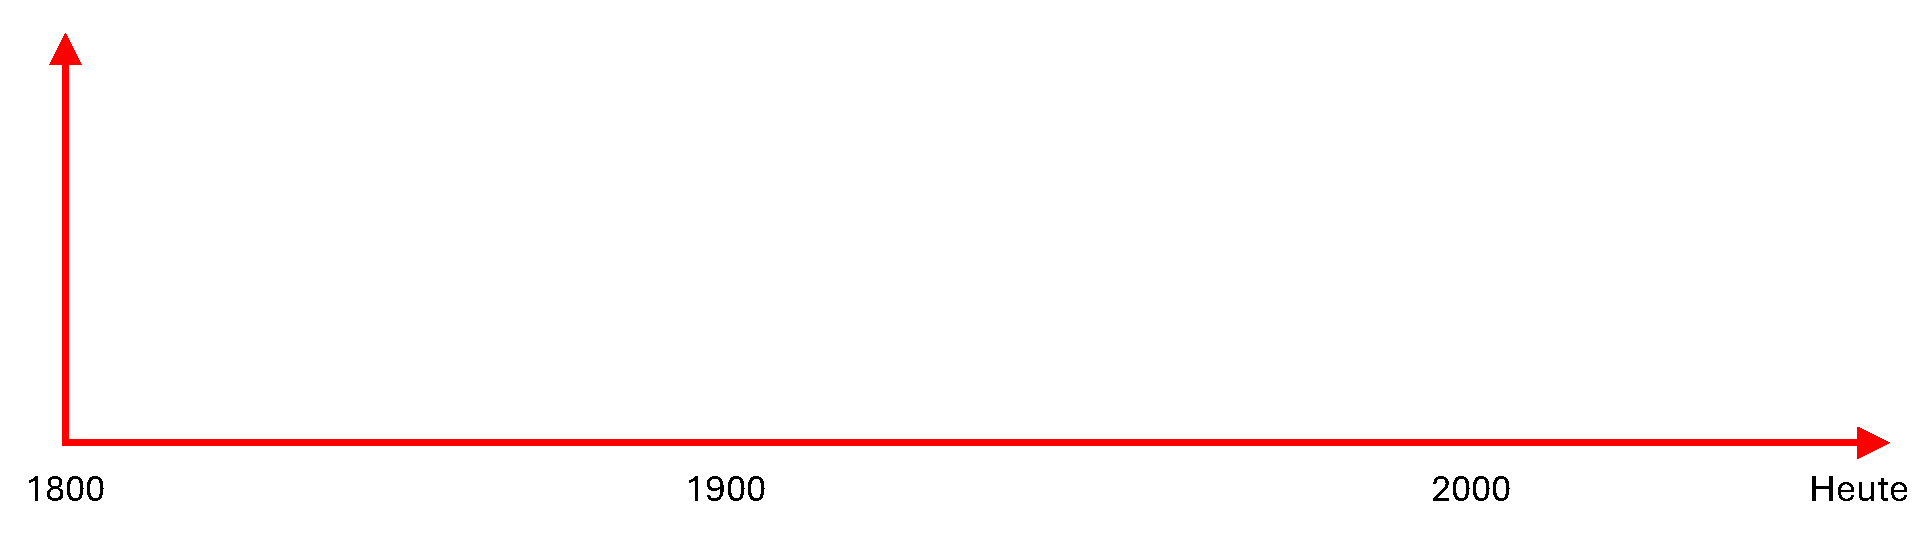
\includegraphics[width=\linewidth]{Private/Images/zeitstrahl}
\end{figure}

\begin{myanswer}
\begin{figure}[H]
\centering
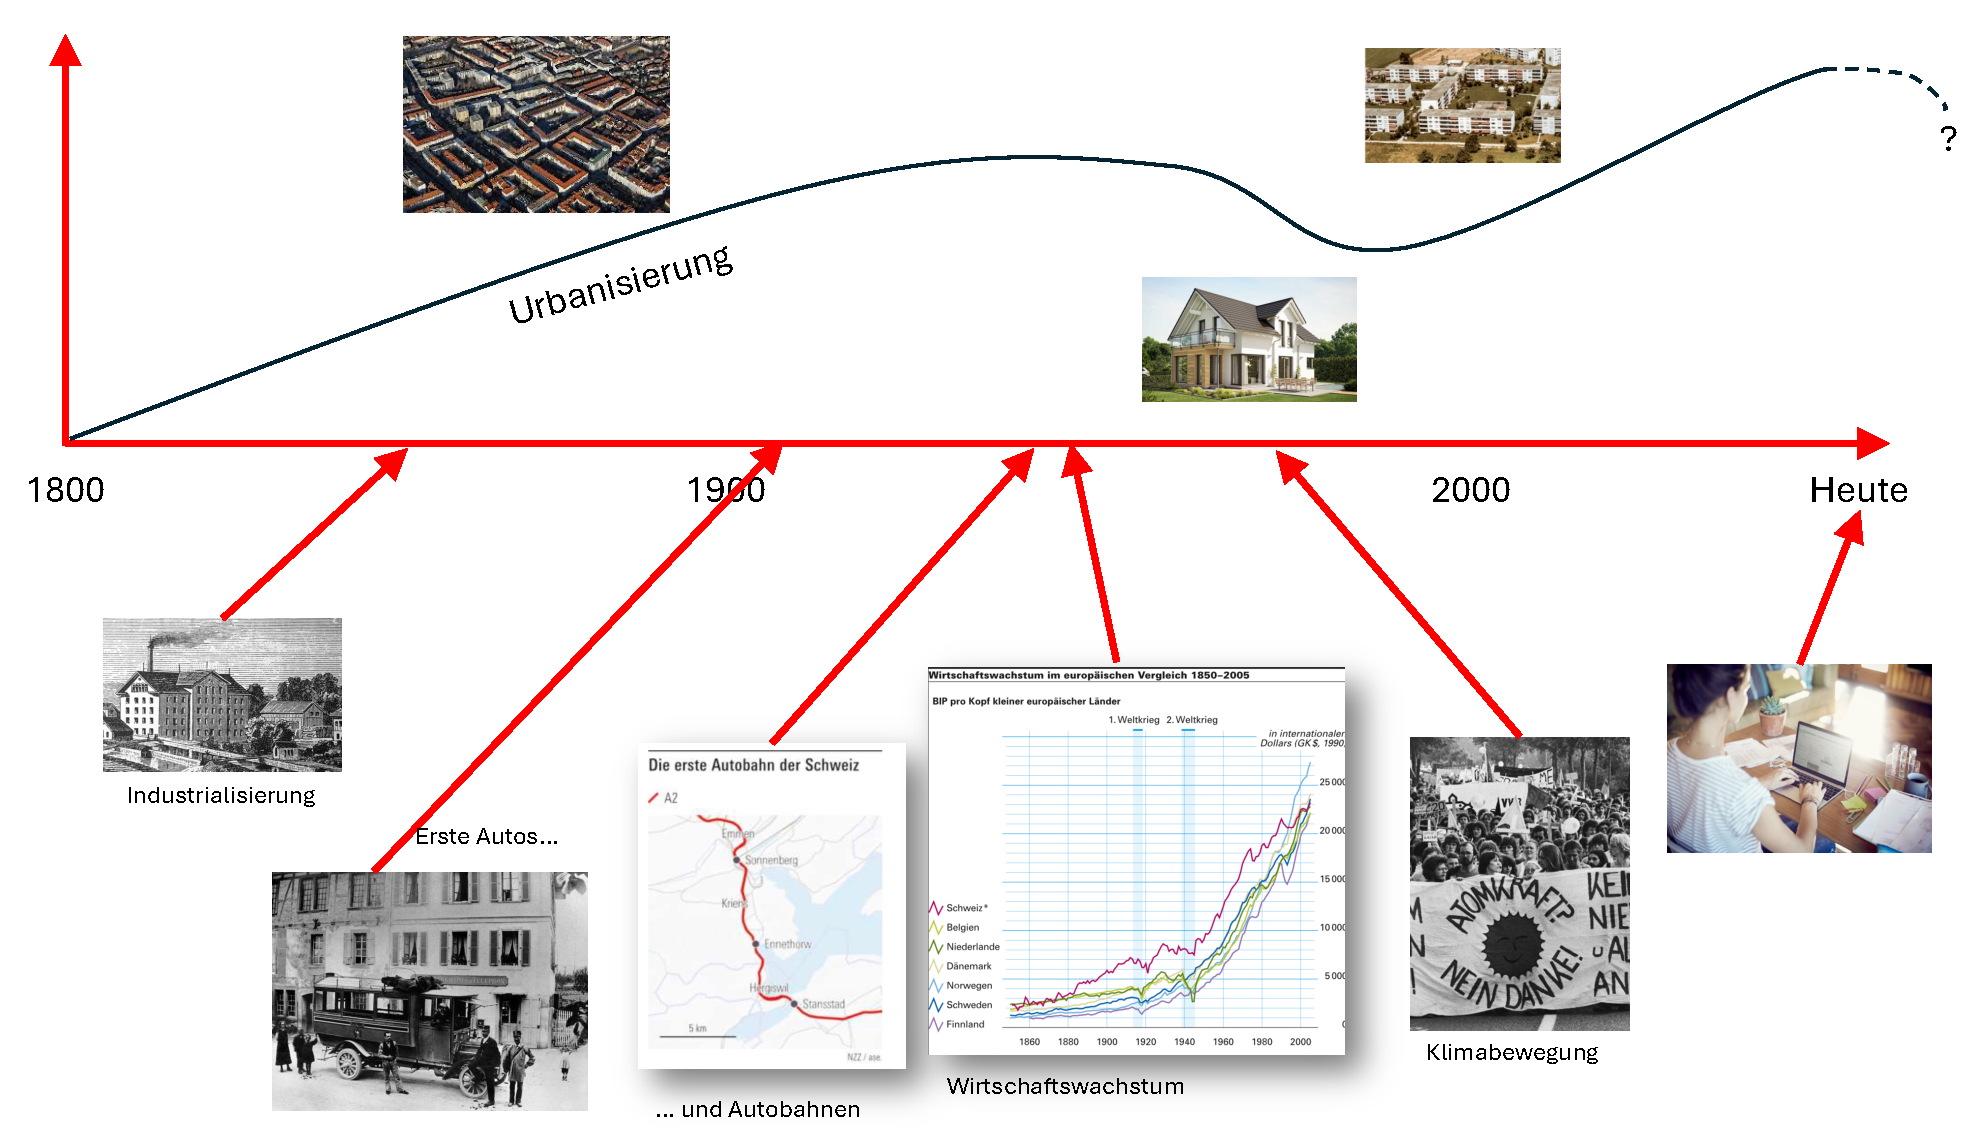
\includegraphics[width=\linewidth]{Private/Images/zeitstrahl-sol}
\end{figure}
\end{myanswer}

\end{myexercise}

\begin{myexercise}[Suburbanisierung (aus \textcite{hep})]
Warum sind seit den 1950er-Jahren immer mehr Menschen in die Kernstädte und in die Umlandgemeinden gezogen? Welches sind die Ursachen und Folgen dieser kleinräumigen Entmischung der demografischen und sozialen Gruppen?


\begin{enumerate}
\item \textbf{Familien} ziehen aus der Kernstadt weg in Umlandgemeinden. Nennen Sie Push- Faktoren und Pull-Faktoren.
\begin{itemize}
\item \textbf{Push-Faktoren}: Was drängt sie aus der Kernstadt weg?
\item \textbf{Pull-Faktoren}: Was zieht sie ins Umland?
\end{itemize}
\item \textbf{Junge Erwerbstätige} (Einzelpersonen oder Paare) ziehen aus dem suburbanen oder ländlichen Raum weg und lassen sich in Kernstädten nieder.
\begin{itemize}
\item \textbf{Push-Faktoren}: Was drängt sie aus dem suburbanen oder ländlichen Raum?
\item \textbf{Pull-Faktoren}: Was zieht sie in die Kernstadt?
\end{itemize}
\end{enumerate}

\begin{myanswer}
\textbf{Familien}: Fortzug aus der Stadt – Zuzug in den suburbanen Raum
\begin{itemize}
    \item Gründe für den Fortzug (Push-Faktoren):
    \begin{itemize}
        \item Unzureichendes Wohnungsangebot
        \item Hohe Mieten, fehlendes oder teures Bauland
        \item Mängel der Bausubstanz und der Wohnumwelt (fehlende Aussicht, geringe Besonnung, kein Garten)
        \item Strassenlärm
        \item Gefahren auf der Strasse für Kinder (Schulweg)
        \item Fehlende Spielplätze in der Nähe der Wohnung
        \item Grosse Distanz zum Wald und zu Naherholungsgebieten
        \item ...
    \end{itemize}
    \item Gründe für den Zuzug ins Umland (Pull-Faktoren):
    \begin{itemize}
        \item Zunehmend höhere Einkommen, mehr Menschen können sich ein Eigenheim leisten
        \item Tiefere Mieten
        \item Relativ grosses Baulandangebot
        \item Grösseres Wohnungsangebot als in der Stadt
        \item Gute Verbindung in die Kernstadt, insbesondere öffentlicher Verkehr
        \item Wunsch nach Wohnen ``im Grünen'', Nähe zu Naherholungsgebieten
        \item ...
    \end{itemize}
\end{itemize}
\textbf{Junge Erwerbstätige} (Einzelpersonen oder Paare), Personen in Ausbildung: Fortzug aus dem suburbanen oder ländlichen Raum – Zuzug in die Stadt
    \begin{itemize}
        \item Gründe für den Fortzug aus dem suburbanen oder ländlichen Raum (Push-Faktoren):
        \begin{itemize}
            \item Geringe Arbeitsmöglichkeiten
            \item Grosse Distanz zum Ausbildungsplatz
            \item Relativ kleines Freizeitangebot
            \item Grosse soziale Kontrolle
            \item ...
        \end{itemize}
        \item Gründe für den Zuzug in die Kernstadt (Pull-Faktoren):
        \begin{itemize}
            \item Relativ hohes Einkommen ermöglicht teurere Mietwohnung in der Stadt
            \item Grosses Wohnungsangebot für Kleinhaushaltungen
            \item Nähe zum Arbeits- oder Ausbildungsplatz
            \item Grosses Versorgungsangebot
            \item Grosses Kultur- und Freizeitangebot
            \item Relativ hohe Anonymität, geringe soziale Kontrolle
            \item ...
        \end{itemize}
    \end{itemize}
\end{myanswer}


\end{myexercise}

\begin{mychallenge}[NZZ-Artikel zu erster Autobahn in der Schweiz]
\begin{figure}[H]
\centering
\colorbox{white}{\includegraphics[width=.9\linewidth]{"Private/Appendix/2024-11-08 Erste Autobahn"}}
\end{figure}
\end{mychallenge}

\begin{mychallenge}[NZZ-Artikel zu 3D-Modell der Stadt Zürich]
\begin{figure}[H]
\centering
\colorbox{white}{\includegraphics[width=.9\linewidth]{"Private/Appendix/2022-04-16 Zürich 3D-Modell"}}
\end{figure}
\end{mychallenge}





\section{Lernziele}
\begin{todolist}
\item Ich kann die Städteentwicklungsphasen Urbanisierung, Suburbanisierung, Periurbanisierung sowie Reurbanisierung und kann diese anhand der demografischen Veränderungen in der Kernstadt, in der Agglomeration sowie im ländlichen Umland charakterisieren. 
\item Ich kann relevante historische Entwicklungen beschreiben (gesellschaftlich, technisch, politisch etc.), welche Städteentwicklungsphasen im 20. Jahrhundert beeinflusst haben.
\item Ich kann beschreieben, welche Faktoren verschiedene Bevölkerungsgruppen (z.B. Familien und junge Erwerbstätige) dazu motivieren, den Wohnort zu wechseln, indem ich relevante Pull- und Push-Faktoren aufliste
\end{todolist}

